\documentclass[10pt]{standalone} 
\usepackage{tikz}
\usetikzlibrary{calc,angles,positioning,intersections,quotes,decorations.markings}
\usepackage{tkz-euclide}
%\usetkzobj{all}
\begin{document}

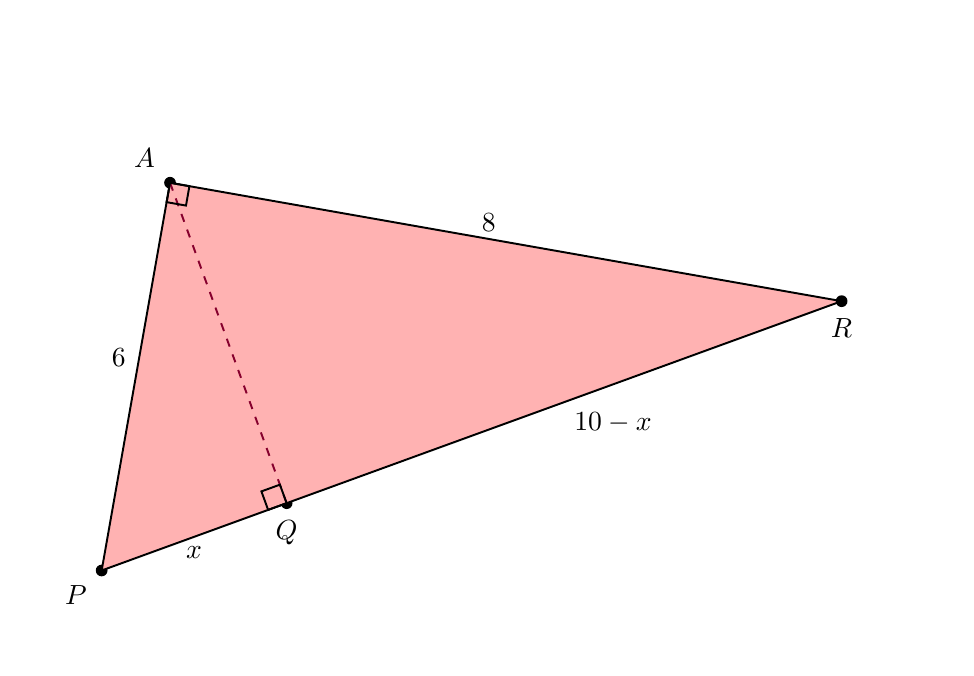
\begin{tikzpicture}[dot/.style={fill,circle,inner sep=1.5pt},line width=.7pt]
\path
  (80:5) node[dot,label=above left:$A$]{} coordinate (A)
  (80:7) coordinate (a)
  (20:9) coordinate (B)
  (20:11) coordinate (b)
  (0:0) node[dot,label=below left:$P$]{} coordinate(P)
  (-100:1)coordinate (e)
  (-160:1)coordinate (f)
  ($(P)!(A)!(B)$)node[dot,label=below:$Q$]{} coordinate(Q);

\path[name path=kline](f)--(b); % First line for intersection
\path[name path=ARline](A)--($(A)!10cm!90:(P)$); % A line normal to pA at point A in the east direction

\path [name intersections={of = ARline and kline, by=R}];
\draw[fill=red!30] (A)--(P)--(R)node[black, dot,label=below:$R$]{}--cycle;
\draw[purple!70!black,dashed] (A)--(Q);

\path (P) -- (Q) node[midway,below] {$x$};
\path (Q) -- (R) node[midway,below right] {$10-x$};
\path (A) -- (R) node[midway,above left] {$8$};
\path (A) -- (P) node[midway,above left] {$6$};

\tkzMarkRightAngle(A,Q,P);
%\tkzMarkAngle[size=0.75cm,color=cyan,mark=||](B,P,A);
%\tkzMarkAngle[size=1cm,color=cyan,mark=|](P,A,Q);
\tkzMarkRightAngle(R,A,P);
\end{tikzpicture}
\end{document}